\chapter{Data Penelitian}

\section{Data Simulasi IES-VE}
Data penelitian ini dapat diakses di \textit{http://bit.ly/DataSkripsiS1Ridhan}

\begin{table}[!h]
	\caption{Data Simulasi IES-VE}
	\label{tbl:A:DataSkripsiRidhan}
	\centering
	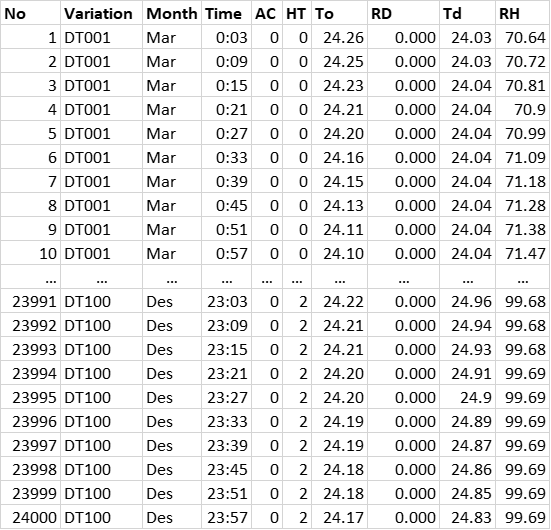
\includegraphics[width=0.75\textwidth]{figures/DataSkripsiRidhan}
\end{table}
\vspace{3em}
\hfill\break
\hfill\break

\section{Bobot-bobot Model Plant JST}
\begin{table}[!h]
	\caption{Bobot-bobot Model Plant JST}
	\label{tbl:A:BobotPlant}
	\centering
	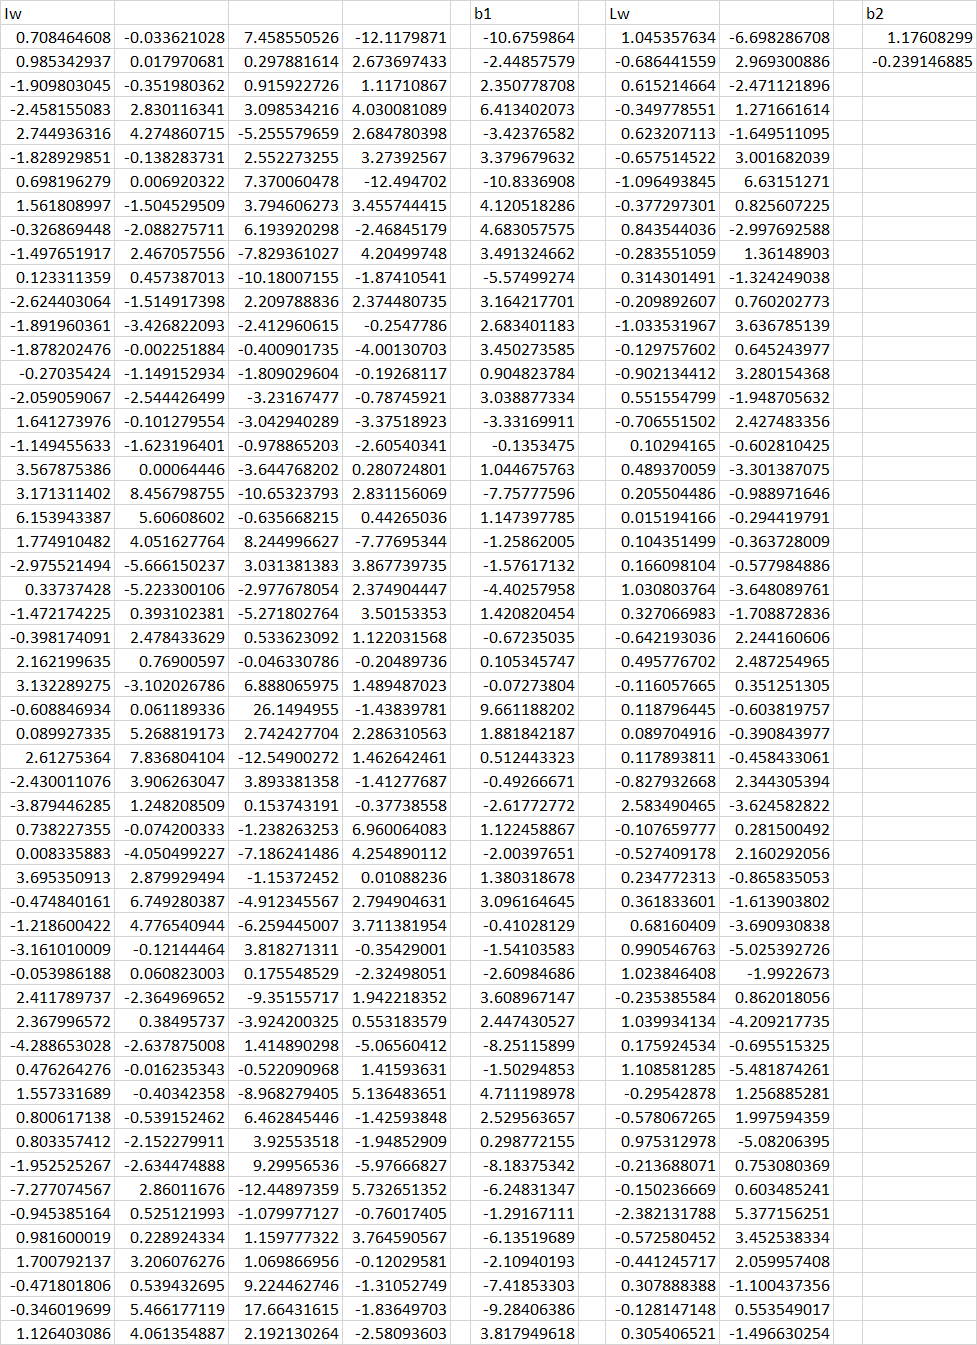
\includegraphics[width=0.95\textwidth]{figures/BobotPlant}
\end{table}
\vspace{2em}

\section{Bobot-bobot Model Emulator JST}
\begin{table}[!h]
	\caption{Bobot-bobot Model Emulator JST}
	\label{tbl:A:BobotEmulator}
	\centering
	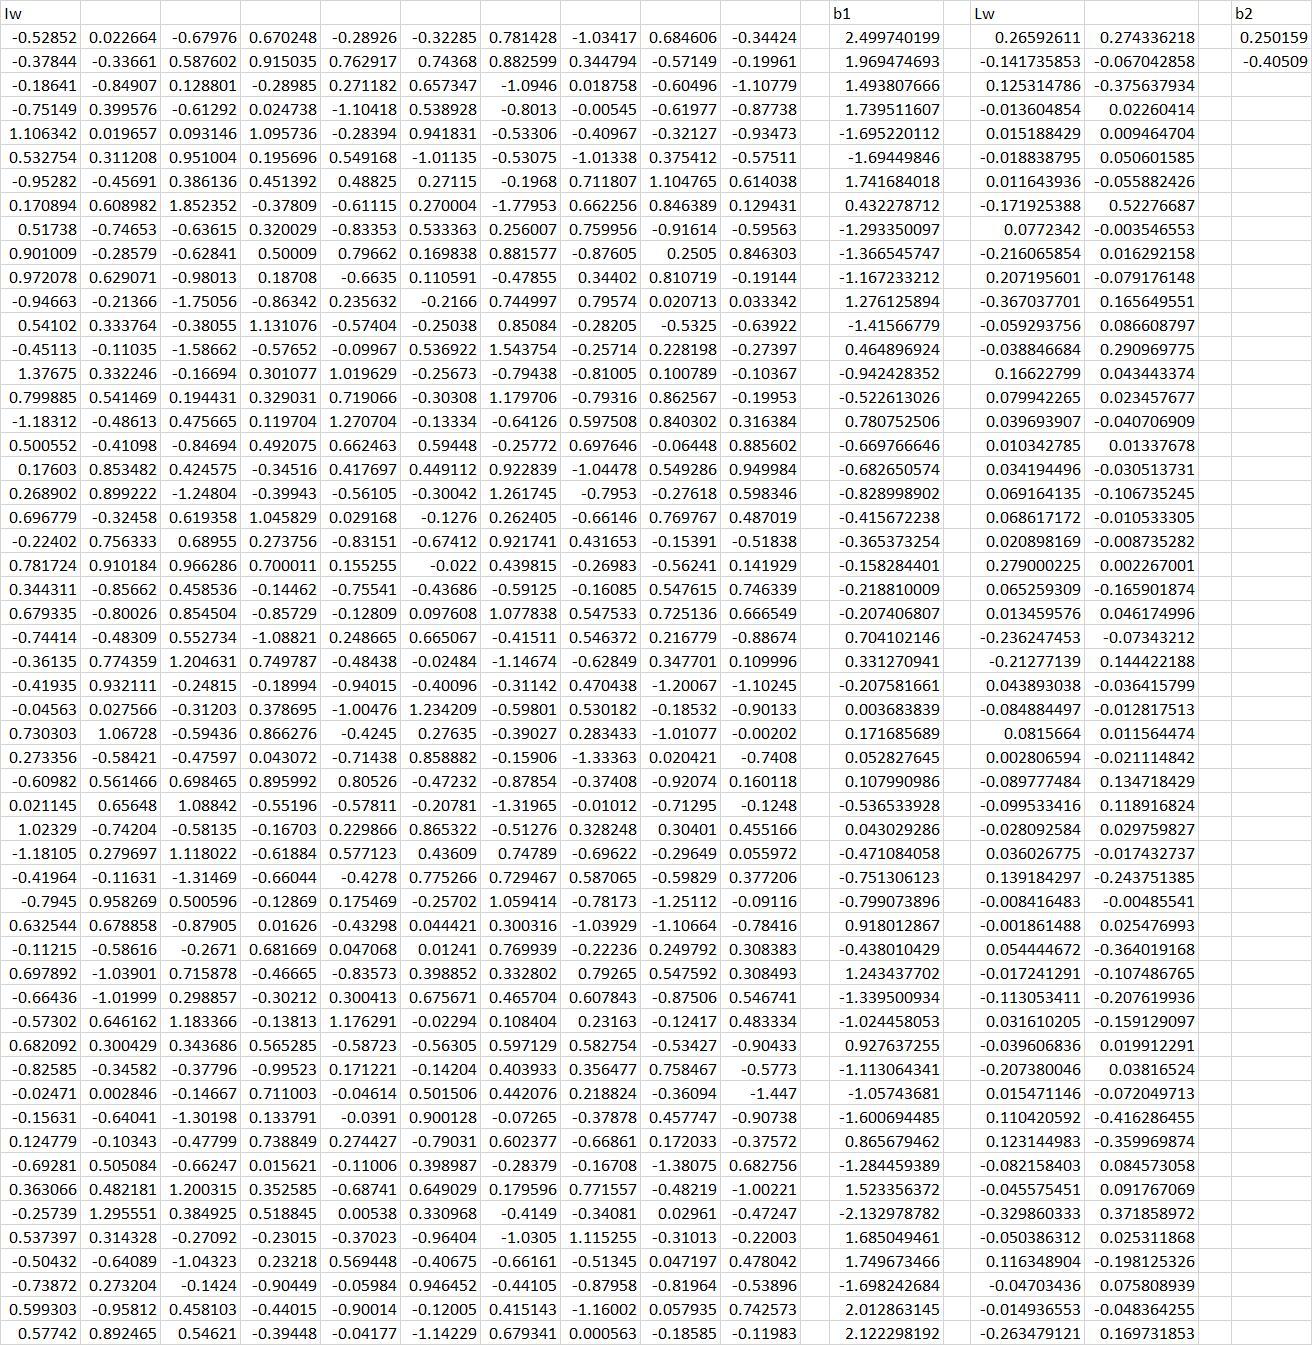
\includegraphics[width=1\textwidth]{figures/BobotEmulator}
\end{table}
\vspace{6em}
\hfill\break

\section{Bobot-bobot Model Kontroler JST}
\begin{table}[!h]
	\caption{Bobot-bobot Model Kontroler JST}
	\label{tbl:A:BobotKontroler}
	\centering
	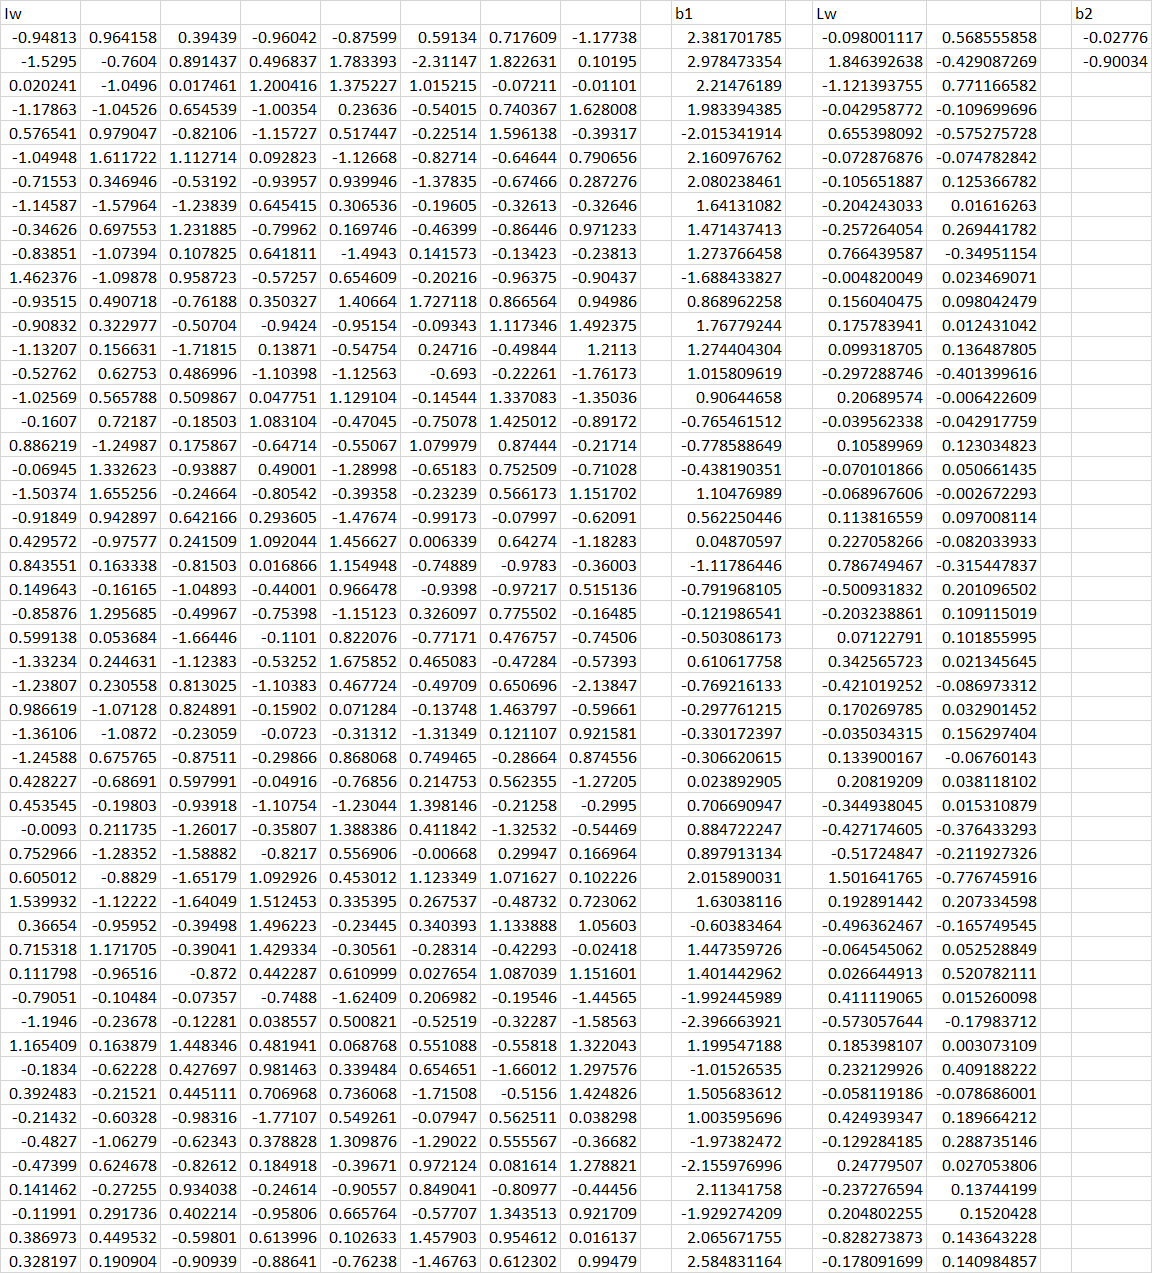
\includegraphics[width=1\textwidth]{figures/BobotKontroler}
\end{table}